\documentclass{article}
\usepackage[utf8]{inputenc}
\usepackage[spanish]{babel}
\usepackage{listings}
\usepackage{graphicx}
\graphicspath{ {images/} }
\usepackage{cite}

\begin{document}

\begin{titlepage}
    \begin{center}
        \vspace*{1cm}
            
        \Huge
        \textbf{Proyecto de Investigación}
            
        \vspace{0.5cm}
        \LARGE
        Taller Noción de la memoria del computador
            
        \vspace{1.5cm}
            
        \textbf{Maria Cristina Vergara Quinchia}
            
        \vfill
            
        \vspace{0.8cm}
            
        \Large
        Despartamento de Ingeniería Electrónica y Telecomunicaciones\\
        Universidad de Antioquia\\
        Medellín\\
        Septiembre de 2020
            
    \end{center}
\end{titlepage}

\tableofcontents
\newpage
\section{Introducción}\label{intro}
Si bien la mayoría de personas ya estamos familiarizadas con las palabra "memoria", que se  define cómo la capacidad para recordar o retener información,se puede formular la siguiente pregunta:que relación tendría la palabra memoria con un computador?Algunos tienen una leve noción de que es y para que sirve este componente dentro de un dispositivo electrónico,en este trabajo se va a abordar el papel que juega la memoria dentro de un computador y se profundizará sobre su concepto,su funcionamiento,los tipos de memorias y sus diferencias.


\section{Contenido} \label{contenido}
A continuación se desarrollarán los puntos propuestos en el taller 
\subsection{Defina que es la memoria del computador}
Las memorias son los dispositivos de almacenamiento de datos e instrucciones en una computadora.\cite{UNT}
La memoria del computador es un dispositivo que guarda la información de forma temporal o sea que almacena información durante un periodo de tiempo,esta información puede ser accedida  por el procesador para ejecutar las instrucciones y realizar las tareas de forma rápida y eficiente.
También se podría definir como un conjunto de celdas de almacenamiento junto con los circuitos asociados que se necesitan para ingresar y sacar la información de almacenamiento.\cite{FIng}

\subsection{Mencione los tipos de memoria que conoce y haga una pequeña descripción de cada tipo.}
Los computadores utilizan varios tipos de memoria con diferentes funciones y características como la velocidad y la capacidad de almacenamiento, las más conocidas son:
\begin{itemize}
\item \textbf{Memoria Caché}:
    La memoria caché consta de tres niveles Nivel 1,Nivel 2 y Nivel 3,actualmente se encuentran localizadas dentro del procesador,esta memoria es mucho más costosa y rápida que la memoria RAM,pueden tener una capacidad hasta de 12 Megabytes.\newline
    Están diseñadas para reducir el tiempo de acceso a la memoria. En la memoria caché se almacenan los datos que se prevé que se utilizarán más habitualmente, de manera que sea posible reducir el número de accesos que debe hacer el procesador a la memoria principal (ya que el tiempo de acceso a la memoria principal siempre es superior al tiempo de acceso a la memoria caché).\cite{Orenga}

    \item \textbf{Memoria RAM((Ramdom Access Memory): }En español Memoria de Acceso Aleatorio,esta memoria es de lectura/escritura, es volátil o sea que su información se pierde cuando no hay suministro de energía.
    
    
    \begin{figure}[h]
    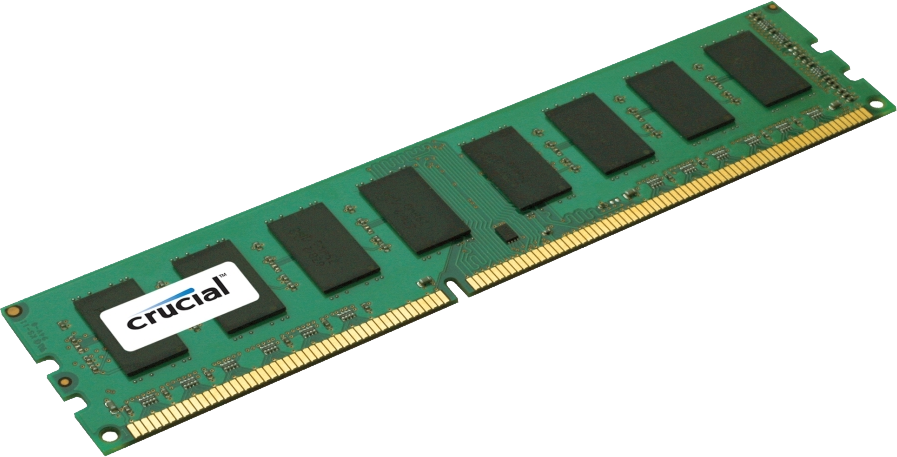
\includegraphics[width=4cm]{memoria.png}
    \centering
    \caption{Memoria RAM}
    \label{fig:memoria}
    \end{figure}
    
    En la Figura (\ref{fig:memoria}), se puede observar una memoria RAM
    
    \item \textbf{Memoria ROM(Read Only Memory)}: En español Memoria de sólo lectura,esta memoria lee la información sin poder modificarla o eliminarla,es una memoria no volátil lo que quiere decir que su información permanece aún si no hay fuente de energía.\newline
    Estas memorias una vez programadas sólo realizan operaciones de lectura. No son volátiles puedenutilizarse para almacenar códigos, generadoras de caracteres, funciones aritméticas complejas, unidades de control microprogramadas, almacenamiento de partes del sistema operativo (BIOS), entre otras.\cite{UNT2}
    
    En la Figura (\ref{fig:rom}), se puede observar una memoria ROM
     \begin{figure}[h]
    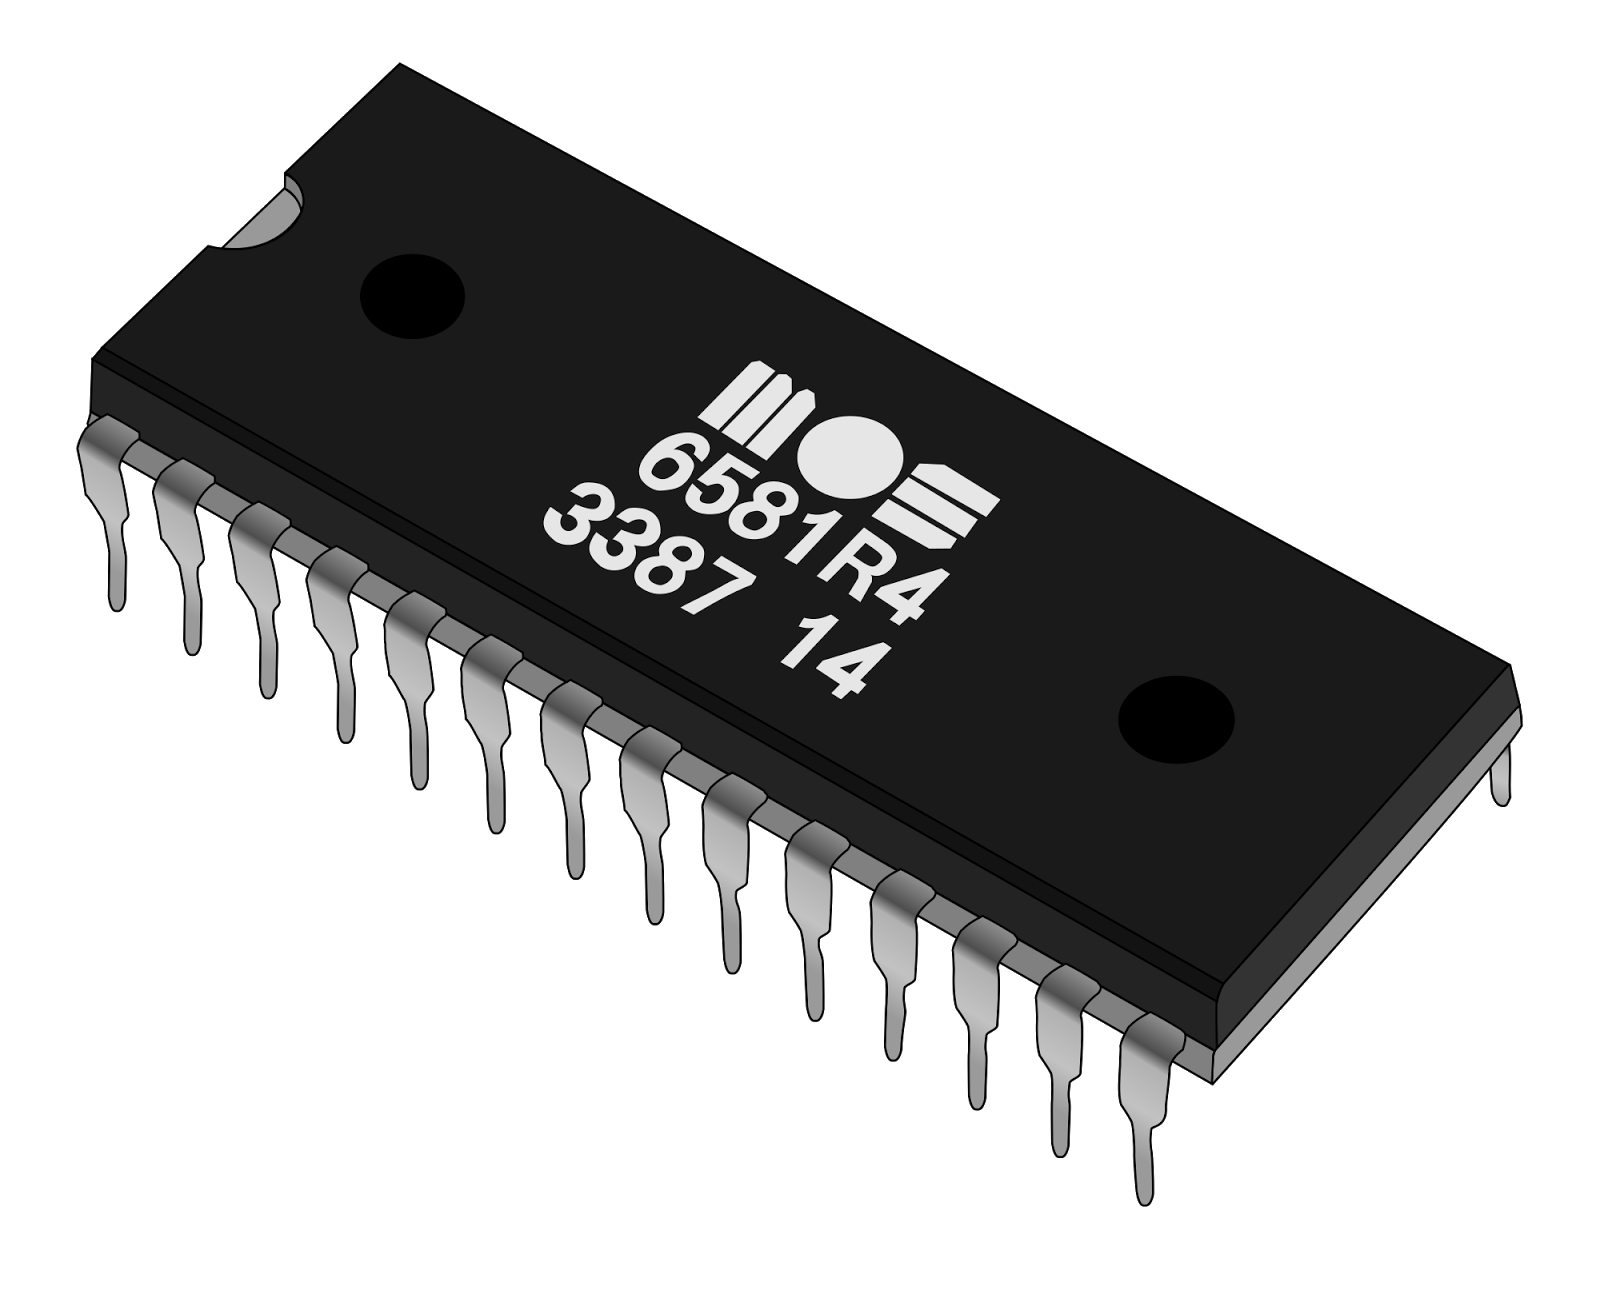
\includegraphics[width=4cm]{rom.png}
    \centering
    \caption{Memoria ROM}
    \label{fig:rom}
    \end{figure}
    
    
\end{itemize}


\subsection{Describa la manera como se gestiona la memoria en un computador}


\subsection{¿Qué hace que una memoria sea más rápida que otra? ¿Por qué esto es importante?}
 \subsection{ Citación}
 











\bibliographystyle{IEEEtran}
\bibliography{references}

\end{document}
